\documentclass[1p]{elsarticle_modified}
%\bibliographystyle{elsarticle-num}

%\usepackage[colorlinks]{hyperref}
%\usepackage{abbrmath_seonhwa} %\Abb, \Ascr, \Acal ,\Abf, \Afrak
\usepackage{amsfonts}
\usepackage{amssymb}
\usepackage{amsmath}
\usepackage{amsthm}
\usepackage{scalefnt}
\usepackage{amsbsy}
\usepackage{kotex}
\usepackage{caption}
\usepackage{subfig}
\usepackage{color}
\usepackage{graphicx}
\usepackage{xcolor} %% white, black, red, green, blue, cyan, magenta, yellow
\usepackage{float}
\usepackage{setspace}
\usepackage{hyperref}

\usepackage{tikz}
\usetikzlibrary{arrows}

\usepackage{multirow}
\usepackage{array} % fixed length table
\usepackage{hhline}

%%%%%%%%%%%%%%%%%%%%%
\makeatletter
\renewcommand*\env@matrix[1][\arraystretch]{%
	\edef\arraystretch{#1}%
	\hskip -\arraycolsep
	\let\@ifnextchar\new@ifnextchar
	\array{*\c@MaxMatrixCols c}}
\makeatother %https://tex.stackexchange.com/questions/14071/how-can-i-increase-the-line-spacing-in-a-matrix
%%%%%%%%%%%%%%%

\usepackage[normalem]{ulem}

\newcommand{\msout}[1]{\ifmmode\text{\sout{\ensuremath{#1}}}\else\sout{#1}\fi}
%SOURCE: \msout is \stkout macro in https://tex.stackexchange.com/questions/20609/strikeout-in-math-mode

\newcommand{\cancel}[1]{
	\ifmmode
	{\color{red}\msout{#1}}
	\else
	{\color{red}\sout{#1}}
	\fi
}

\newcommand{\add}[1]{
	{\color{blue}\uwave{#1}}
}

\newcommand{\replace}[2]{
	\ifmmode
	{\color{red}\msout{#1}}{\color{blue}\uwave{#2}}
	\else
	{\color{red}\sout{#1}}{\color{blue}\uwave{#2}}
	\fi
}

\newcommand{\Sol}{\mathcal{S}} %segment
\newcommand{\D}{D} %diagram
\newcommand{\A}{\mathcal{A}} %arc


%%%%%%%%%%%%%%%%%%%%%%%%%%%%%5 test

\def\sl{\operatorname{\textup{SL}}(2,\Cbb)}
\def\psl{\operatorname{\textup{PSL}}(2,\Cbb)}
\def\quan{\mkern 1mu \triangleright \mkern 1mu}

\theoremstyle{definition}
\newtheorem{thm}{Theorem}[section]
\newtheorem{prop}[thm]{Proposition}
\newtheorem{lem}[thm]{Lemma}
\newtheorem{ques}[thm]{Question}
\newtheorem{cor}[thm]{Corollary}
\newtheorem{defn}[thm]{Definition}
\newtheorem{exam}[thm]{Example}
\newtheorem{rmk}[thm]{Remark}
\newtheorem{alg}[thm]{Algorithm}

\newcommand{\I}{\sqrt{-1}}
\begin{document}

%\begin{frontmatter}
%
%\title{Boundary parabolic representations of knots up to 8 crossings}
%
%%% Group authors per affiliation:
%\author{Yunhi Cho} 
%\address{Department of Mathematics, University of Seoul, Seoul, Korea}
%\ead{yhcho@uos.ac.kr}
%
%
%\author{Seonhwa Kim} %\fnref{s_kim}}
%\address{Center for Geometry and Physics, Institute for Basic Science, Pohang, 37673, Korea}
%\ead{ryeona17@ibs.re.kr}
%
%\author{Hyuk Kim}
%\address{Department of Mathematical Sciences, Seoul National University, Seoul 08826, Korea}
%\ead{hyukkim@snu.ac.kr}
%
%\author{Seokbeom Yoon}
%\address{Department of Mathematical Sciences, Seoul National University, Seoul, 08826,  Korea}
%\ead{sbyoon15@snu.ac.kr}
%
%\begin{abstract}
%We find all boundary parabolic representation of knots up to 8 crossings.
%
%\end{abstract}
%\begin{keyword}
%    \MSC[2010] 57M25 
%\end{keyword}
%
%\end{frontmatter}

%\linenumbers
%\tableofcontents
%
\newcommand\colored[1]{\textcolor{white}{\rule[-0.35ex]{0.8em}{1.4ex}}\kern-0.8em\color{red} #1}%
%\newcommand\colored[1]{\textcolor{white}{ #1}\kern-2.17ex	\textcolor{white}{ #1}\kern-1.81ex	\textcolor{white}{ #1}\kern-2.15ex\color{red}#1	}

{\Large $\underline{12a_{0934}~(K12a_{0934})}$}

\setlength{\tabcolsep}{10pt}
\renewcommand{\arraystretch}{1.6}
\vspace{1cm}\begin{tabular}{m{100pt}>{\centering\arraybackslash}m{274pt}}
\multirow{5}{120pt}{
	\centering
	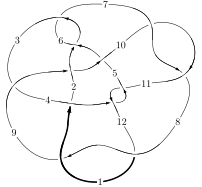
\includegraphics[width=112pt]{../../../GIT/diagram.site/Diagrams/png/1735_12a_0934.png}\\
\ \ \ A knot diagram\footnotemark}&
\allowdisplaybreaks
\textbf{Linearized knot diagam} \\
\cline{2-2}
 &
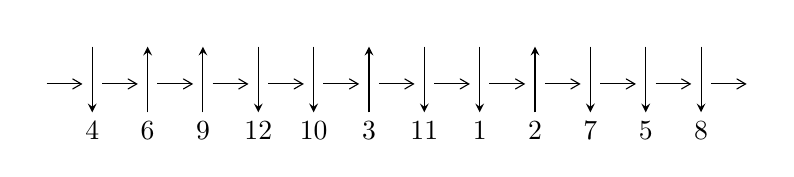
\begin{tikzpicture}[x=20pt, y=17pt]
	% nodes
	\node (C0) at (0, 0) {};
	\node (C1) at (1, 0) {};
	\node (C1U) at (1, +1) {};
	\node (C1D) at (1, -1) {4};

	\node (C2) at (2, 0) {};
	\node (C2U) at (2, +1) {};
	\node (C2D) at (2, -1) {6};

	\node (C3) at (3, 0) {};
	\node (C3U) at (3, +1) {};
	\node (C3D) at (3, -1) {9};

	\node (C4) at (4, 0) {};
	\node (C4U) at (4, +1) {};
	\node (C4D) at (4, -1) {12};

	\node (C5) at (5, 0) {};
	\node (C5U) at (5, +1) {};
	\node (C5D) at (5, -1) {10};

	\node (C6) at (6, 0) {};
	\node (C6U) at (6, +1) {};
	\node (C6D) at (6, -1) {3};

	\node (C7) at (7, 0) {};
	\node (C7U) at (7, +1) {};
	\node (C7D) at (7, -1) {11};

	\node (C8) at (8, 0) {};
	\node (C8U) at (8, +1) {};
	\node (C8D) at (8, -1) {1};

	\node (C9) at (9, 0) {};
	\node (C9U) at (9, +1) {};
	\node (C9D) at (9, -1) {2};

	\node (C10) at (10, 0) {};
	\node (C10U) at (10, +1) {};
	\node (C10D) at (10, -1) {7};

	\node (C11) at (11, 0) {};
	\node (C11U) at (11, +1) {};
	\node (C11D) at (11, -1) {5};

	\node (C12) at (12, 0) {};
	\node (C12U) at (12, +1) {};
	\node (C12D) at (12, -1) {8};
	\node (C13) at (13, 0) {};

	% arrows
	\draw[->,>={angle 60}]
	(C0) edge (C1) (C1) edge (C2) (C2) edge (C3) (C3) edge (C4) (C4) edge (C5) (C5) edge (C6) (C6) edge (C7) (C7) edge (C8) (C8) edge (C9) (C9) edge (C10) (C10) edge (C11) (C11) edge (C12) (C12) edge (C13) ;	\draw[->,>=stealth]
	(C1U) edge (C1D) (C2D) edge (C2U) (C3D) edge (C3U) (C4U) edge (C4D) (C5U) edge (C5D) (C6D) edge (C6U) (C7U) edge (C7D) (C8U) edge (C8D) (C9D) edge (C9U) (C10U) edge (C10D) (C11U) edge (C11D) (C12U) edge (C12D) ;
	\end{tikzpicture} \\
\hhline{~~} \\& 
\textbf{Solving Sequence} \\ \cline{2-2} 
 &
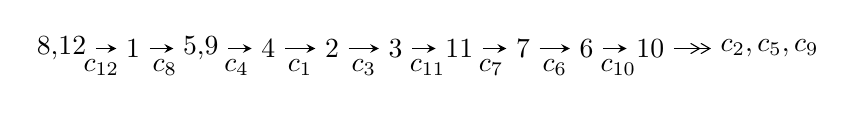
\begin{tikzpicture}[x=23pt, y=7pt]
	% node
	\node (A0) at (-1/8, 0) {8,12};
	\node (A1) at (1, 0) {1};
	\node (A2) at (33/16, 0) {5,9};
	\node (A3) at (25/8, 0) {4};
	\node (A4) at (33/8, 0) {2};
	\node (A5) at (41/8, 0) {3};
	\node (A6) at (49/8, 0) {11};
	\node (A7) at (57/8, 0) {7};
	\node (A8) at (65/8, 0) {6};
	\node (A9) at (73/8, 0) {10};
	\node (C1) at (1/2, -1) {$c_{12}$};
	\node (C2) at (3/2, -1) {$c_{8}$};
	\node (C3) at (21/8, -1) {$c_{4}$};
	\node (C4) at (29/8, -1) {$c_{1}$};
	\node (C5) at (37/8, -1) {$c_{3}$};
	\node (C6) at (45/8, -1) {$c_{11}$};
	\node (C7) at (53/8, -1) {$c_{7}$};
	\node (C8) at (61/8, -1) {$c_{6}$};
	\node (C9) at (69/8, -1) {$c_{10}$};
	\node (A10) at (11, 0) {$c_{2},c_{5},c_{9}$};

	% edge
	\draw[->,>=stealth]	
	(A0) edge (A1) (A1) edge (A2) (A2) edge (A3) (A3) edge (A4) (A4) edge (A5) (A5) edge (A6) (A6) edge (A7) (A7) edge (A8) (A8) edge (A9) ;
	\draw[->>,>={angle 60}]	
	(A9) edge (A10);
\end{tikzpicture} \\ 

\end{tabular} \\

\footnotetext{
The image of knot diagram is generated by the software ``\textbf{Draw programme}" developed by Andrew Bartholomew(\url{http://www.layer8.co.uk/maths/draw/index.htm\#Running-draw}), where we modified some parts for our purpose(\url{https://github.com/CATsTAILs/LinksPainter}).
}\phantom \\ \newline 
\centering \textbf{Ideals for irreducible components\footnotemark of $X_{\text{par}}$} 
 
\begin{align*}
I^u_{1}&=\langle 
-8.17977\times10^{836} u^{142}-2.61309\times10^{836} u^{141}+\cdots+1.56473\times10^{838} b+1.90810\times10^{838},\\
\phantom{I^u_{1}}&\phantom{= \langle  }1.66586\times10^{840} u^{142}-1.26723\times10^{840} u^{141}+\cdots+2.10456\times10^{841} a+3.71585\times10^{842},\\
\phantom{I^u_{1}}&\phantom{= \langle  }u^{143}-47 u^{141}+\cdots+364 u+269\rangle \\
I^u_{2}&=\langle 
-1.71204\times10^{17} u^{25}+3.05492\times10^{16} u^{24}+\cdots+5.91030\times10^{16} b-5.58176\times10^{17},\\
\phantom{I^u_{2}}&\phantom{= \langle  }-5.21337\times10^{18} u^{25}-1.64739\times10^{18} u^{24}+\cdots+2.95515\times10^{17} a-6.14328\times10^{18},\;u^{26}+u^{25}+\cdots+u+1\rangle \\
\\
\end{align*}
\raggedright * 2 irreducible components of $\dim_{\mathbb{C}}=0$, with total 169 representations.\\
\footnotetext{All coefficients of polynomials are rational numbers. But the coefficients are sometimes approximated in decimal forms when there is not enough margin.}
\newpage
\renewcommand{\arraystretch}{1}
\centering \section*{I. $I^u_{1}= \langle -8.18\times10^{836} u^{142}-2.61\times10^{836} u^{141}+\cdots+1.56\times10^{838} b+1.91\times10^{838},\;1.67\times10^{840} u^{142}-1.27\times10^{840} u^{141}+\cdots+2.10\times10^{841} a+3.72\times10^{842},\;u^{143}-47 u^{141}+\cdots+364 u+269 \rangle$}
\flushleft \textbf{(i) Arc colorings}\\
\begin{tabular}{m{7pt} m{180pt} m{7pt} m{180pt} }
\flushright $a_{8}=$&$\begin{pmatrix}0\\u\end{pmatrix}$ \\
\flushright $a_{12}=$&$\begin{pmatrix}1\\0\end{pmatrix}$ \\
\flushright $a_{1}=$&$\begin{pmatrix}1\\u^2\end{pmatrix}$ \\
\flushright $a_{5}=$&$\begin{pmatrix}-0.0791551 u^{142}+0.0602135 u^{141}+\cdots+30.8779 u-17.6562\\0.0522761 u^{142}+0.0167000 u^{141}+\cdots-11.6519 u-1.21945\end{pmatrix}$ \\
\flushright $a_{9}=$&$\begin{pmatrix}- u\\- u^3+u\end{pmatrix}$ \\
\flushright $a_{4}=$&$\begin{pmatrix}-0.0268790 u^{142}+0.0769135 u^{141}+\cdots+19.2260 u-18.8757\\0.0522761 u^{142}+0.0167000 u^{141}+\cdots-11.6519 u-1.21945\end{pmatrix}$ \\
\flushright $a_{2}=$&$\begin{pmatrix}-0.0610283 u^{142}+0.124610 u^{141}+\cdots-57.5228 u-42.7584\\-0.00749442 u^{142}+0.0569378 u^{141}+\cdots-15.5122 u-13.7115\end{pmatrix}$ \\
\flushright $a_{3}=$&$\begin{pmatrix}-0.0816065 u^{142}+0.0545344 u^{141}+\cdots+38.9646 u-14.3467\\0.0492722 u^{142}+0.0126226 u^{141}+\cdots-8.52288 u+0.271532\end{pmatrix}$ \\
\flushright $a_{11}=$&$\begin{pmatrix}-0.0324903 u^{142}+0.0277336 u^{141}+\cdots+4.34640 u+2.11357\\-0.0977073 u^{142}-0.113732 u^{141}+\cdots+81.8388 u+36.8451\end{pmatrix}$ \\
\flushright $a_{7}=$&$\begin{pmatrix}0.0416650 u^{142}-0.100566 u^{141}+\cdots+49.8985 u+25.4480\\0.0806253 u^{142}-0.0132788 u^{141}+\cdots-13.2509 u+3.21127\end{pmatrix}$ \\
\flushright $a_{6}=$&$\begin{pmatrix}0.117340 u^{142}-0.163859 u^{141}+\cdots+61.4302 u+43.4479\\0.0498635 u^{142}+0.00880346 u^{141}+\cdots-9.16620 u-0.0498885\end{pmatrix}$ \\
\flushright $a_{10}=$&$\begin{pmatrix}-0.0155967 u^{142}-0.0605104 u^{141}+\cdots+40.6021 u+20.4252\\0.0372287 u^{142}-0.0727408 u^{141}+\cdots+14.6857 u+19.7369\end{pmatrix}$\\&\end{tabular}
\flushleft \textbf{(ii) Obstruction class $= -1$}\\~\\
\flushleft \textbf{(iii) Cusp Shapes $= -0.00649429 u^{142}+0.580777 u^{141}+\cdots-330.566 u-189.922$}\\~\\
\newpage\renewcommand{\arraystretch}{1}
\flushleft \textbf{(iv) u-Polynomials at the component}\newline \\
\begin{tabular}{m{50pt}|m{274pt}}
Crossings & \hspace{64pt}u-Polynomials at each crossing \\
\hline $$\begin{aligned}c_{1}\end{aligned}$$&$\begin{aligned}
&5(5 u^{143}-74 u^{142}+\cdots+39 u-1)
\end{aligned}$\\
\hline $$\begin{aligned}c_{2},c_{6}\end{aligned}$$&$\begin{aligned}
&u^{143}-6 u^{142}+\cdots-1576 u+172
\end{aligned}$\\
\hline $$\begin{aligned}c_{3}\end{aligned}$$&$\begin{aligned}
&u^{143}- u^{142}+\cdots-165495 u+28517
\end{aligned}$\\
\hline $$\begin{aligned}c_{4},c_{11}\end{aligned}$$&$\begin{aligned}
&u^{143}+2 u^{142}+\cdots+5 u+1
\end{aligned}$\\
\hline $$\begin{aligned}c_{5}\end{aligned}$$&$\begin{aligned}
&u^{143}-5 u^{142}+\cdots+29545559 u+4359035
\end{aligned}$\\
\hline $$\begin{aligned}c_{7},c_{10}\end{aligned}$$&$\begin{aligned}
&5(5 u^{143}+12 u^{142}+\cdots-18368 u+853)
\end{aligned}$\\
\hline $$\begin{aligned}c_{8},c_{12}\end{aligned}$$&$\begin{aligned}
&u^{143}-47 u^{141}+\cdots+364 u+269
\end{aligned}$\\
\hline $$\begin{aligned}c_{9}\end{aligned}$$&$\begin{aligned}
&5(5 u^{143}+13 u^{142}+\cdots+1.70137\times10^{7} u+3351097)
\end{aligned}$\\
\hline
\end{tabular}\\~\\
\newpage\renewcommand{\arraystretch}{1}
\flushleft \textbf{(v) Riley Polynomials at the component}\newline \\
\begin{tabular}{m{50pt}|m{274pt}}
Crossings & \hspace{64pt}Riley Polynomials at each crossing \\
\hline $$\begin{aligned}c_{1}\end{aligned}$$&$\begin{aligned}
&25(25 y^{143}+604 y^{142}+\cdots+121 y-1)
\end{aligned}$\\
\hline $$\begin{aligned}c_{2},c_{6}\end{aligned}$$&$\begin{aligned}
&y^{143}-76 y^{142}+\cdots+959512 y-29584
\end{aligned}$\\
\hline $$\begin{aligned}c_{3}\end{aligned}$$&$\begin{aligned}
&y^{143}+41 y^{142}+\cdots-38361226787 y-813219289
\end{aligned}$\\
\hline $$\begin{aligned}c_{4},c_{11}\end{aligned}$$&$\begin{aligned}
&y^{143}+86 y^{142}+\cdots+121 y-1
\end{aligned}$\\
\hline $$\begin{aligned}c_{5}\end{aligned}$$&$\begin{aligned}
&y^{143}+23 y^{142}+\cdots+104456910942711 y-19001186131225
\end{aligned}$\\
\hline $$\begin{aligned}c_{7},c_{10}\end{aligned}$$&$\begin{aligned}
&25(25 y^{143}-2914 y^{142}+\cdots+1.04124\times10^{8} y-727609)
\end{aligned}$\\
\hline $$\begin{aligned}c_{8},c_{12}\end{aligned}$$&$\begin{aligned}
&y^{143}-94 y^{142}+\cdots+5651838 y-72361
\end{aligned}$\\
\hline $$\begin{aligned}c_{9}\end{aligned}$$&$\begin{aligned}
&25\\
&\cdot(25 y^{143}-1509 y^{142}+\cdots+228455902797875 y-11229851103409)
\end{aligned}$\\
\hline
\end{tabular}\\~\\
\newpage\flushleft \textbf{(vi) Complex Volumes and Cusp Shapes}
$$\begin{array}{c|c|c}  
\text{Solutions to }I^u_{1}& \I (\text{vol} + \sqrt{-1}CS) & \text{Cusp shape}\\
 \hline 
\begin{aligned}
u &= \phantom{-}0.953441 + 0.280184 I \\
a &= \phantom{-}1.396460 + 0.048949 I \\
b &= \phantom{-}0.191314 - 0.190861 I\end{aligned}
 & -2.83635 - 4.15021 I & \phantom{-0.000000 } 0 \\ \hline\begin{aligned}
u &= \phantom{-}0.953441 - 0.280184 I \\
a &= \phantom{-}1.396460 - 0.048949 I \\
b &= \phantom{-}0.191314 + 0.190861 I\end{aligned}
 & -2.83635 + 4.15021 I & \phantom{-0.000000 } 0 \\ \hline\begin{aligned}
u &= -1.010390 + 0.030646 I \\
a &= -0.11325 - 2.01286 I \\
b &= \phantom{-}0.034402 - 0.865725 I\end{aligned}
 & -0.001877 - 0.442384 I & \phantom{-0.000000 } 0 \\ \hline\begin{aligned}
u &= -1.010390 - 0.030646 I \\
a &= -0.11325 + 2.01286 I \\
b &= \phantom{-}0.034402 + 0.865725 I\end{aligned}
 & -0.001877 + 0.442384 I & \phantom{-0.000000 } 0 \\ \hline\begin{aligned}
u &= -0.987219 + 0.014942 I \\
a &= -0.76824 + 2.79757 I \\
b &= -0.130585 - 1.246220 I\end{aligned}
 & \phantom{-}0.106125 + 0.616101 I & \phantom{-0.000000 } 0 \\ \hline\begin{aligned}
u &= -0.987219 - 0.014942 I \\
a &= -0.76824 - 2.79757 I \\
b &= -0.130585 + 1.246220 I\end{aligned}
 & \phantom{-}0.106125 - 0.616101 I & \phantom{-0.000000 } 0 \\ \hline\begin{aligned}
u &= -0.783799 + 0.643101 I \\
a &= -1.145450 - 0.671197 I \\
b &= \phantom{-}0.159109 + 0.679276 I\end{aligned}
 & -1.32608 - 0.55698 I & \phantom{-0.000000 } 0 \\ \hline\begin{aligned}
u &= -0.783799 - 0.643101 I \\
a &= -1.145450 + 0.671197 I \\
b &= \phantom{-}0.159109 - 0.679276 I\end{aligned}
 & -1.32608 + 0.55698 I & \phantom{-0.000000 } 0 \\ \hline\begin{aligned}
u &= \phantom{-}0.981212 + 0.039484 I \\
a &= -0.156321 - 0.796016 I \\
b &= -0.53247 + 2.38239 I\end{aligned}
 & \phantom{-}2.58358 - 4.22251 I & \phantom{-0.000000 } 0 \\ \hline\begin{aligned}
u &= \phantom{-}0.981212 - 0.039484 I \\
a &= -0.156321 + 0.796016 I \\
b &= -0.53247 - 2.38239 I\end{aligned}
 & \phantom{-}2.58358 + 4.22251 I & \phantom{-0.000000 } 0\\
 \hline 
 \end{array}$$\newpage$$\begin{array}{c|c|c}  
\text{Solutions to }I^u_{1}& \I (\text{vol} + \sqrt{-1}CS) & \text{Cusp shape}\\
 \hline 
\begin{aligned}
u &= \phantom{-}0.168376 + 1.010290 I \\
a &= -0.403018 + 1.329770 I \\
b &= \phantom{-}0.434505 - 1.198880 I\end{aligned}
 & \phantom{-}6.76187 + 3.68604 I & \phantom{-0.000000 } 0 \\ \hline\begin{aligned}
u &= \phantom{-}0.168376 - 1.010290 I \\
a &= -0.403018 - 1.329770 I \\
b &= \phantom{-}0.434505 + 1.198880 I\end{aligned}
 & \phantom{-}6.76187 - 3.68604 I & \phantom{-0.000000 } 0 \\ \hline\begin{aligned}
u &= -1.024100 + 0.082462 I \\
a &= \phantom{-}0.999925 - 0.454984 I \\
b &= \phantom{-}0.489112 + 0.884310 I\end{aligned}
 & -2.25844 + 0.52198 I & \phantom{-0.000000 } 0 \\ \hline\begin{aligned}
u &= -1.024100 - 0.082462 I \\
a &= \phantom{-}0.999925 + 0.454984 I \\
b &= \phantom{-}0.489112 - 0.884310 I\end{aligned}
 & -2.25844 - 0.52198 I & \phantom{-0.000000 } 0 \\ \hline\begin{aligned}
u &= \phantom{-}0.982228 + 0.303791 I \\
a &= -0.235058 + 1.247610 I \\
b &= -0.150528 - 0.716160 I\end{aligned}
 & \phantom{-}0.85063 - 2.71396 I & \phantom{-0.000000 } 0 \\ \hline\begin{aligned}
u &= \phantom{-}0.982228 - 0.303791 I \\
a &= -0.235058 - 1.247610 I \\
b &= -0.150528 + 0.716160 I\end{aligned}
 & \phantom{-}0.85063 + 2.71396 I & \phantom{-0.000000 } 0 \\ \hline\begin{aligned}
u &= \phantom{-}0.962958 + 0.098303 I \\
a &= \phantom{-}0.267266 + 0.030566 I \\
b &= \phantom{-}0.77834 + 1.61887 I\end{aligned}
 & \phantom{-}2.51023 + 3.69294 I & \phantom{-0.000000 } 0 \\ \hline\begin{aligned}
u &= \phantom{-}0.962958 - 0.098303 I \\
a &= \phantom{-}0.267266 - 0.030566 I \\
b &= \phantom{-}0.77834 - 1.61887 I\end{aligned}
 & \phantom{-}2.51023 - 3.69294 I & \phantom{-0.000000 } 0 \\ \hline\begin{aligned}
u &= -0.089637 + 1.034830 I \\
a &= \phantom{-}0.19639 - 1.60103 I \\
b &= \phantom{-}0.172723 + 1.291120 I\end{aligned}
 & \phantom{-}8.09161 - 7.20861 I & \phantom{-0.000000 } 0 \\ \hline\begin{aligned}
u &= -0.089637 - 1.034830 I \\
a &= \phantom{-}0.19639 + 1.60103 I \\
b &= \phantom{-}0.172723 - 1.291120 I\end{aligned}
 & \phantom{-}8.09161 + 7.20861 I & \phantom{-0.000000 } 0\\
 \hline 
 \end{array}$$\newpage$$\begin{array}{c|c|c}  
\text{Solutions to }I^u_{1}& \I (\text{vol} + \sqrt{-1}CS) & \text{Cusp shape}\\
 \hline 
\begin{aligned}
u &= \phantom{-}0.110001 + 0.954827 I \\
a &= -0.26538 + 1.47531 I \\
b &= -0.097892 - 1.271540 I\end{aligned}
 & \phantom{-}4.82132 - 2.58137 I & \phantom{-0.000000 } 0 \\ \hline\begin{aligned}
u &= \phantom{-}0.110001 - 0.954827 I \\
a &= -0.26538 - 1.47531 I \\
b &= -0.097892 + 1.271540 I\end{aligned}
 & \phantom{-}4.82132 + 2.58137 I & \phantom{-0.000000 } 0 \\ \hline\begin{aligned}
u &= -1.003690 + 0.323417 I \\
a &= -0.312210 - 0.087098 I \\
b &= -1.027220 - 0.536386 I\end{aligned}
 & \phantom{-}1.12598 + 2.47967 I & \phantom{-0.000000 } 0 \\ \hline\begin{aligned}
u &= -1.003690 - 0.323417 I \\
a &= -0.312210 + 0.087098 I \\
b &= -1.027220 + 0.536386 I\end{aligned}
 & \phantom{-}1.12598 - 2.47967 I & \phantom{-0.000000 } 0 \\ \hline\begin{aligned}
u &= -0.890332 + 0.317106 I \\
a &= \phantom{-}0.247103 + 0.210024 I \\
b &= -0.80279 - 1.54479 I\end{aligned}
 & \phantom{-}2.38525 + 3.10272 I & \phantom{-0.000000 } 0 \\ \hline\begin{aligned}
u &= -0.890332 - 0.317106 I \\
a &= \phantom{-}0.247103 - 0.210024 I \\
b &= -0.80279 + 1.54479 I\end{aligned}
 & \phantom{-}2.38525 - 3.10272 I & \phantom{-0.000000 } 0 \\ \hline\begin{aligned}
u &= -1.063350 + 0.252145 I \\
a &= -0.41624 - 1.54398 I \\
b &= -0.410990 + 1.303960 I\end{aligned}
 & -3.17300 + 3.96230 I & \phantom{-0.000000 } 0 \\ \hline\begin{aligned}
u &= -1.063350 - 0.252145 I \\
a &= -0.41624 + 1.54398 I \\
b &= -0.410990 - 1.303960 I\end{aligned}
 & -3.17300 - 3.96230 I & \phantom{-0.000000 } 0 \\ \hline\begin{aligned}
u &= -1.025570 + 0.384280 I \\
a &= -0.651829 - 1.021830 I \\
b &= -0.98342 + 1.42689 I\end{aligned}
 & -1.80463 + 5.84988 I & \phantom{-0.000000 } 0 \\ \hline\begin{aligned}
u &= -1.025570 - 0.384280 I \\
a &= -0.651829 + 1.021830 I \\
b &= -0.98342 - 1.42689 I\end{aligned}
 & -1.80463 - 5.84988 I & \phantom{-0.000000 } 0\\
 \hline 
 \end{array}$$\newpage$$\begin{array}{c|c|c}  
\text{Solutions to }I^u_{1}& \I (\text{vol} + \sqrt{-1}CS) & \text{Cusp shape}\\
 \hline 
\begin{aligned}
u &= \phantom{-}1.006130 + 0.461398 I \\
a &= \phantom{-}1.014620 - 0.660352 I \\
b &= \phantom{-}0.474415 + 1.220100 I\end{aligned}
 & \phantom{-}6.42005 - 5.22402 I & \phantom{-0.000000 } 0 \\ \hline\begin{aligned}
u &= \phantom{-}1.006130 - 0.461398 I \\
a &= \phantom{-}1.014620 + 0.660352 I \\
b &= \phantom{-}0.474415 - 1.220100 I\end{aligned}
 & \phantom{-}6.42005 + 5.22402 I & \phantom{-0.000000 } 0 \\ \hline\begin{aligned}
u &= \phantom{-}1.104300 + 0.136126 I \\
a &= \phantom{-}1.18282 - 1.18140 I \\
b &= \phantom{-}0.704634 + 1.081220 I\end{aligned}
 & -5.06245 - 4.49479 I & \phantom{-0.000000 } 0 \\ \hline\begin{aligned}
u &= \phantom{-}1.104300 - 0.136126 I \\
a &= \phantom{-}1.18282 + 1.18140 I \\
b &= \phantom{-}0.704634 - 1.081220 I\end{aligned}
 & -5.06245 + 4.49479 I & \phantom{-0.000000 } 0 \\ \hline\begin{aligned}
u &= \phantom{-}0.723528 + 0.513111 I \\
a &= -1.42116 + 0.78634 I \\
b &= \phantom{-}0.137355 + 0.053830 I\end{aligned}
 & \phantom{-}0.61991 - 9.62524 I & \phantom{-0.000000 } 0 \\ \hline\begin{aligned}
u &= \phantom{-}0.723528 - 0.513111 I \\
a &= -1.42116 - 0.78634 I \\
b &= \phantom{-}0.137355 - 0.053830 I\end{aligned}
 & \phantom{-}0.61991 + 9.62524 I & \phantom{-0.000000 } 0 \\ \hline\begin{aligned}
u &= -0.332280 + 0.813049 I \\
a &= -1.24577 - 1.60100 I \\
b &= \phantom{-}0.323420 + 0.654559 I\end{aligned}
 & -1.181230 - 0.629478 I & \phantom{-0.000000 } 0 \\ \hline\begin{aligned}
u &= -0.332280 - 0.813049 I \\
a &= -1.24577 + 1.60100 I \\
b &= \phantom{-}0.323420 - 0.654559 I\end{aligned}
 & -1.181230 + 0.629478 I & \phantom{-0.000000 } 0 \\ \hline\begin{aligned}
u &= -0.220671 + 0.840921 I \\
a &= -1.01507 - 1.12871 I \\
b &= \phantom{-}0.313244 + 1.159900 I\end{aligned}
 & \phantom{-}0.48502 - 1.68739 I & \phantom{-0.000000 } 0 \\ \hline\begin{aligned}
u &= -0.220671 - 0.840921 I \\
a &= -1.01507 + 1.12871 I \\
b &= \phantom{-}0.313244 - 1.159900 I\end{aligned}
 & \phantom{-}0.48502 + 1.68739 I & \phantom{-0.000000 } 0\\
 \hline 
 \end{array}$$\newpage$$\begin{array}{c|c|c}  
\text{Solutions to }I^u_{1}& \I (\text{vol} + \sqrt{-1}CS) & \text{Cusp shape}\\
 \hline 
\begin{aligned}
u &= \phantom{-}1.101010 + 0.295639 I \\
a &= -1.89392 + 0.97993 I \\
b &= -0.283702 - 0.936183 I\end{aligned}
 & \phantom{-}1.12905 - 1.16214 I & \phantom{-0.000000 } 0 \\ \hline\begin{aligned}
u &= \phantom{-}1.101010 - 0.295639 I \\
a &= -1.89392 - 0.97993 I \\
b &= -0.283702 + 0.936183 I\end{aligned}
 & \phantom{-}1.12905 + 1.16214 I & \phantom{-0.000000 } 0 \\ \hline\begin{aligned}
u &= -0.963608 + 0.612550 I \\
a &= \phantom{-}0.73453 + 1.31416 I \\
b &= \phantom{-}0.83474 - 1.22537 I\end{aligned}
 & \phantom{-}2.77422 + 10.96720 I & \phantom{-0.000000 } 0 \\ \hline\begin{aligned}
u &= -0.963608 - 0.612550 I \\
a &= \phantom{-}0.73453 - 1.31416 I \\
b &= \phantom{-}0.83474 + 1.22537 I\end{aligned}
 & \phantom{-}2.77422 - 10.96720 I & \phantom{-0.000000 } 0 \\ \hline\begin{aligned}
u &= -0.847432\phantom{ +0.000000I} \\
a &= -0.655806\phantom{ +0.000000I} \\
b &= -0.337970\phantom{ +0.000000I}\end{aligned}
 & -1.26647\phantom{ +0.000000I} & \phantom{-0.000000 } 0 \\ \hline\begin{aligned}
u &= -1.152880 + 0.066472 I \\
a &= \phantom{-}0.632318 + 1.250730 I \\
b &= \phantom{-}0.481285 - 1.196730 I\end{aligned}
 & -3.38562 - 0.59244 I & \phantom{-0.000000 } 0 \\ \hline\begin{aligned}
u &= -1.152880 - 0.066472 I \\
a &= \phantom{-}0.632318 - 1.250730 I \\
b &= \phantom{-}0.481285 + 1.196730 I\end{aligned}
 & -3.38562 + 0.59244 I & \phantom{-0.000000 } 0 \\ \hline\begin{aligned}
u &= -0.705574 + 0.917719 I \\
a &= \phantom{-}0.649939 + 0.783705 I \\
b &= -0.512130 - 1.146120 I\end{aligned}
 & \phantom{-}3.72031 - 5.32101 I & \phantom{-0.000000 } 0 \\ \hline\begin{aligned}
u &= -0.705574 - 0.917719 I \\
a &= \phantom{-}0.649939 - 0.783705 I \\
b &= -0.512130 + 1.146120 I\end{aligned}
 & \phantom{-}3.72031 + 5.32101 I & \phantom{-0.000000 } 0 \\ \hline\begin{aligned}
u &= -0.581728 + 0.599275 I \\
a &= \phantom{-}0.153970 + 0.705721 I \\
b &= -0.195329 + 0.058974 I\end{aligned}
 & -1.23695 + 1.89390 I & \phantom{-0.000000 } 0\\
 \hline 
 \end{array}$$\newpage$$\begin{array}{c|c|c}  
\text{Solutions to }I^u_{1}& \I (\text{vol} + \sqrt{-1}CS) & \text{Cusp shape}\\
 \hline 
\begin{aligned}
u &= -0.581728 - 0.599275 I \\
a &= \phantom{-}0.153970 - 0.705721 I \\
b &= -0.195329 - 0.058974 I\end{aligned}
 & -1.23695 - 1.89390 I & \phantom{-0.000000 } 0 \\ \hline\begin{aligned}
u &= \phantom{-}0.832800 + 0.047985 I \\
a &= -2.20444 + 1.00568 I \\
b &= -0.237110 - 0.562946 I\end{aligned}
 & \phantom{-}2.37529 - 0.91245 I & \phantom{-0.000000 } 0 \\ \hline\begin{aligned}
u &= \phantom{-}0.832800 - 0.047985 I \\
a &= -2.20444 - 1.00568 I \\
b &= -0.237110 + 0.562946 I\end{aligned}
 & \phantom{-}2.37529 + 0.91245 I & \phantom{-0.000000 } 0 \\ \hline\begin{aligned}
u &= \phantom{-}1.155320 + 0.169801 I \\
a &= -1.14673 + 1.41366 I \\
b &= -0.579450 - 1.180900 I\end{aligned}
 & -2.06102 - 10.51710 I & \phantom{-0.000000 } 0 \\ \hline\begin{aligned}
u &= \phantom{-}1.155320 - 0.169801 I \\
a &= -1.14673 - 1.41366 I \\
b &= -0.579450 + 1.180900 I\end{aligned}
 & -2.06102 + 10.51710 I & \phantom{-0.000000 } 0 \\ \hline\begin{aligned}
u &= \phantom{-}1.133480 + 0.316419 I \\
a &= \phantom{-}0.949414 - 0.757396 I \\
b &= \phantom{-}1.044660 + 0.873227 I\end{aligned}
 & -3.90278 - 4.96723 I & \phantom{-0.000000 } 0 \\ \hline\begin{aligned}
u &= \phantom{-}1.133480 - 0.316419 I \\
a &= \phantom{-}0.949414 + 0.757396 I \\
b &= \phantom{-}1.044660 - 0.873227 I\end{aligned}
 & -3.90278 + 4.96723 I & \phantom{-0.000000 } 0 \\ \hline\begin{aligned}
u &= -1.118630 + 0.396045 I \\
a &= -0.230661 - 0.577414 I \\
b &= -0.198672 + 0.029125 I\end{aligned}
 & -0.764453 - 0.954747 I & \phantom{-0.000000 } 0 \\ \hline\begin{aligned}
u &= -1.118630 - 0.396045 I \\
a &= -0.230661 + 0.577414 I \\
b &= -0.198672 - 0.029125 I\end{aligned}
 & -0.764453 + 0.954747 I & \phantom{-0.000000 } 0 \\ \hline\begin{aligned}
u &= -0.118570 + 1.188670 I \\
a &= \phantom{-}0.34493 - 1.37248 I \\
b &= -0.430334 + 1.207880 I\end{aligned}
 & \phantom{-}1.22717 + 7.53373 I & \phantom{-0.000000 } 0\\
 \hline 
 \end{array}$$\newpage$$\begin{array}{c|c|c}  
\text{Solutions to }I^u_{1}& \I (\text{vol} + \sqrt{-1}CS) & \text{Cusp shape}\\
 \hline 
\begin{aligned}
u &= -0.118570 - 1.188670 I \\
a &= \phantom{-}0.34493 + 1.37248 I \\
b &= -0.430334 - 1.207880 I\end{aligned}
 & \phantom{-}1.22717 - 7.53373 I & \phantom{-0.000000 } 0 \\ \hline\begin{aligned}
u &= \phantom{-}0.677140 + 0.409760 I \\
a &= -1.43195 + 1.61775 I \\
b &= -0.806800 - 0.408804 I\end{aligned}
 & \phantom{-}1.207770 + 0.495852 I & \phantom{-0.000000 } 0 \\ \hline\begin{aligned}
u &= \phantom{-}0.677140 - 0.409760 I \\
a &= -1.43195 - 1.61775 I \\
b &= -0.806800 + 0.408804 I\end{aligned}
 & \phantom{-}1.207770 - 0.495852 I & \phantom{-0.000000 } 0 \\ \hline\begin{aligned}
u &= \phantom{-}0.157111 + 0.734759 I \\
a &= -0.1312460 + 0.0400883 I \\
b &= \phantom{-}0.577568 - 0.342079 I\end{aligned}
 & \phantom{-}3.03390 + 4.61751 I & \phantom{-0.000000 } 0 \\ \hline\begin{aligned}
u &= \phantom{-}0.157111 - 0.734759 I \\
a &= -0.1312460 - 0.0400883 I \\
b &= \phantom{-}0.577568 + 0.342079 I\end{aligned}
 & \phantom{-}3.03390 - 4.61751 I & \phantom{-0.000000 } 0 \\ \hline\begin{aligned}
u &= \phantom{-}1.174530 + 0.474847 I \\
a &= \phantom{-}0.966589 - 0.577097 I \\
b &= \phantom{-}0.397074 + 0.610269 I\end{aligned}
 & -3.00556 - 4.48240 I & \phantom{-0.000000 } 0 \\ \hline\begin{aligned}
u &= \phantom{-}1.174530 - 0.474847 I \\
a &= \phantom{-}0.966589 + 0.577097 I \\
b &= \phantom{-}0.397074 - 0.610269 I\end{aligned}
 & -3.00556 + 4.48240 I & \phantom{-0.000000 } 0 \\ \hline\begin{aligned}
u &= \phantom{-}1.146160 + 0.564297 I \\
a &= -0.661465 + 0.725930 I \\
b &= -0.653511 - 0.462588 I\end{aligned}
 & \phantom{-}0.31844 - 9.32512 I & \phantom{-0.000000 } 0 \\ \hline\begin{aligned}
u &= \phantom{-}1.146160 - 0.564297 I \\
a &= -0.661465 - 0.725930 I \\
b &= -0.653511 + 0.462588 I\end{aligned}
 & \phantom{-}0.31844 + 9.32512 I & \phantom{-0.000000 } 0 \\ \hline\begin{aligned}
u &= -1.253640 + 0.264323 I \\
a &= \phantom{-}0.0344833 - 0.0027068 I \\
b &= \phantom{-}1.55923 + 0.24399 I\end{aligned}
 & -7.06638 + 5.97890 I & \phantom{-0.000000 } 0\\
 \hline 
 \end{array}$$\newpage$$\begin{array}{c|c|c}  
\text{Solutions to }I^u_{1}& \I (\text{vol} + \sqrt{-1}CS) & \text{Cusp shape}\\
 \hline 
\begin{aligned}
u &= -1.253640 - 0.264323 I \\
a &= \phantom{-}0.0344833 + 0.0027068 I \\
b &= \phantom{-}1.55923 - 0.24399 I\end{aligned}
 & -7.06638 - 5.97890 I & \phantom{-0.000000 } 0 \\ \hline\begin{aligned}
u &= \phantom{-}1.143220 + 0.644015 I \\
a &= -0.465776 + 1.130320 I \\
b &= -0.246405 - 1.101650 I\end{aligned}
 & \phantom{-}1.46034 - 2.65575 I & \phantom{-0.000000 } 0 \\ \hline\begin{aligned}
u &= \phantom{-}1.143220 - 0.644015 I \\
a &= -0.465776 - 1.130320 I \\
b &= -0.246405 + 1.101650 I\end{aligned}
 & \phantom{-}1.46034 + 2.65575 I & \phantom{-0.000000 } 0 \\ \hline\begin{aligned}
u &= \phantom{-}0.513860 + 0.455627 I \\
a &= -0.627920 + 0.129495 I \\
b &= \phantom{-}0.832741 - 0.680431 I\end{aligned}
 & \phantom{-}1.52959 - 4.07522 I & \phantom{-0.000000 } 0 \\ \hline\begin{aligned}
u &= \phantom{-}0.513860 - 0.455627 I \\
a &= -0.627920 - 0.129495 I \\
b &= \phantom{-}0.832741 + 0.680431 I\end{aligned}
 & \phantom{-}1.52959 + 4.07522 I & \phantom{-0.000000 } 0 \\ \hline\begin{aligned}
u &= -1.287890 + 0.357625 I \\
a &= -1.018530 - 0.249437 I \\
b &= -0.425248 + 1.101860 I\end{aligned}
 & \phantom{-}4.46110 + 2.31741 I & \phantom{-0.000000 } 0 \\ \hline\begin{aligned}
u &= -1.287890 - 0.357625 I \\
a &= -1.018530 + 0.249437 I \\
b &= -0.425248 - 1.101860 I\end{aligned}
 & \phantom{-}4.46110 - 2.31741 I & \phantom{-0.000000 } 0 \\ \hline\begin{aligned}
u &= -1.299090 + 0.339174 I \\
a &= \phantom{-}0.0071974 - 0.0201440 I \\
b &= -1.40845 - 0.18824 I\end{aligned}
 & -4.22308 + 12.77700 I & \phantom{-0.000000 } 0 \\ \hline\begin{aligned}
u &= -1.299090 - 0.339174 I \\
a &= \phantom{-}0.0071974 + 0.0201440 I \\
b &= -1.40845 + 0.18824 I\end{aligned}
 & -4.22308 - 12.77700 I & \phantom{-0.000000 } 0 \\ \hline\begin{aligned}
u &= -0.617090 + 0.191281 I \\
a &= \phantom{-}1.54730 + 0.50118 I \\
b &= \phantom{-}1.098090 - 0.569613 I\end{aligned}
 & \phantom{-}3.27057 - 0.27522 I & \phantom{-0.000000 } 0\\
 \hline 
 \end{array}$$\newpage$$\begin{array}{c|c|c}  
\text{Solutions to }I^u_{1}& \I (\text{vol} + \sqrt{-1}CS) & \text{Cusp shape}\\
 \hline 
\begin{aligned}
u &= -0.617090 - 0.191281 I \\
a &= \phantom{-}1.54730 - 0.50118 I \\
b &= \phantom{-}1.098090 + 0.569613 I\end{aligned}
 & \phantom{-}3.27057 + 0.27522 I & \phantom{-0.000000 } 0 \\ \hline\begin{aligned}
u &= \phantom{-}1.348760 + 0.191117 I \\
a &= \phantom{-}0.0473985 - 0.0250200 I \\
b &= -1.110880 + 0.147139 I\end{aligned}
 & -8.27484 - 1.14930 I & \phantom{-0.000000 } 0 \\ \hline\begin{aligned}
u &= \phantom{-}1.348760 - 0.191117 I \\
a &= \phantom{-}0.0473985 + 0.0250200 I \\
b &= -1.110880 - 0.147139 I\end{aligned}
 & -8.27484 + 1.14930 I & \phantom{-0.000000 } 0 \\ \hline\begin{aligned}
u &= \phantom{-}0.401349 + 0.495221 I \\
a &= -0.43868 - 3.17924 I \\
b &= \phantom{-}0.118252 + 1.088580 I\end{aligned}
 & \phantom{-}0.87637 - 1.28498 I & \phantom{-0.000000 } 0 \\ \hline\begin{aligned}
u &= \phantom{-}0.401349 - 0.495221 I \\
a &= -0.43868 + 3.17924 I \\
b &= \phantom{-}0.118252 - 1.088580 I\end{aligned}
 & \phantom{-}0.87637 + 1.28498 I & \phantom{-0.000000 } 0 \\ \hline\begin{aligned}
u &= -0.039875 + 1.366560 I \\
a &= -0.338713 + 1.335540 I \\
b &= \phantom{-}0.430615 - 1.191370 I\end{aligned}
 & \phantom{-}4.05091 + 13.22030 I & \phantom{-0.000000 } 0 \\ \hline\begin{aligned}
u &= -0.039875 - 1.366560 I \\
a &= -0.338713 - 1.335540 I \\
b &= \phantom{-}0.430615 + 1.191370 I\end{aligned}
 & \phantom{-}4.05091 - 13.22030 I & \phantom{-0.000000 } 0 \\ \hline\begin{aligned}
u &= -1.369400 + 0.083168 I \\
a &= \phantom{-}0.253440 - 0.220657 I \\
b &= \phantom{-}0.870309 - 0.616922 I\end{aligned}
 & -6.48596 + 1.39889 I & \phantom{-0.000000 } 0 \\ \hline\begin{aligned}
u &= -1.369400 - 0.083168 I \\
a &= \phantom{-}0.253440 + 0.220657 I \\
b &= \phantom{-}0.870309 + 0.616922 I\end{aligned}
 & -6.48596 - 1.39889 I & \phantom{-0.000000 } 0 \\ \hline\begin{aligned}
u &= \phantom{-}1.263360 + 0.538364 I \\
a &= -0.804710 + 1.037870 I \\
b &= -0.74435 - 1.24554 I\end{aligned}
 & \phantom{-}3.33005 - 9.19163 I & \phantom{-0.000000 } 0\\
 \hline 
 \end{array}$$\newpage$$\begin{array}{c|c|c}  
\text{Solutions to }I^u_{1}& \I (\text{vol} + \sqrt{-1}CS) & \text{Cusp shape}\\
 \hline 
\begin{aligned}
u &= \phantom{-}1.263360 - 0.538364 I \\
a &= -0.804710 - 1.037870 I \\
b &= -0.74435 + 1.24554 I\end{aligned}
 & \phantom{-}3.33005 + 9.19163 I & \phantom{-0.000000 } 0 \\ \hline\begin{aligned}
u &= \phantom{-}1.266690 + 0.532028 I \\
a &= -0.408116 + 0.923419 I \\
b &= -0.231903 - 1.182370 I\end{aligned}
 & \phantom{-}1.47092 - 2.63775 I & \phantom{-0.000000 } 0 \\ \hline\begin{aligned}
u &= \phantom{-}1.266690 - 0.532028 I \\
a &= -0.408116 - 0.923419 I \\
b &= -0.231903 + 1.182370 I\end{aligned}
 & \phantom{-}1.47092 + 2.63775 I & \phantom{-0.000000 } 0 \\ \hline\begin{aligned}
u &= \phantom{-}1.331500 + 0.398460 I \\
a &= \phantom{-}0.136812 - 0.247068 I \\
b &= -1.003340 + 0.420358 I\end{aligned}
 & -6.13084 - 3.78973 I & \phantom{-0.000000 } 0 \\ \hline\begin{aligned}
u &= \phantom{-}1.331500 - 0.398460 I \\
a &= \phantom{-}0.136812 + 0.247068 I \\
b &= -1.003340 - 0.420358 I\end{aligned}
 & -6.13084 + 3.78973 I & \phantom{-0.000000 } 0 \\ \hline\begin{aligned}
u &= \phantom{-}0.473594 + 0.356276 I \\
a &= \phantom{-}0.355076 - 0.981933 I \\
b &= -0.11273 + 1.53753 I\end{aligned}
 & \phantom{-}8.23718 + 1.34496 I & \phantom{-}6.93628 + 6.15710 I \\ \hline\begin{aligned}
u &= \phantom{-}0.473594 - 0.356276 I \\
a &= \phantom{-}0.355076 + 0.981933 I \\
b &= -0.11273 - 1.53753 I\end{aligned}
 & \phantom{-}8.23718 - 1.34496 I & \phantom{-}6.93628 - 6.15710 I \\ \hline\begin{aligned}
u &= -1.31723 + 0.52281 I \\
a &= -1.088310 - 0.825424 I \\
b &= -0.409585 + 1.197380 I\end{aligned}
 & \phantom{-}4.21891 + 12.73810 I & \phantom{-0.000000 } 0 \\ \hline\begin{aligned}
u &= -1.31723 - 0.52281 I \\
a &= -1.088310 + 0.825424 I \\
b &= -0.409585 - 1.197380 I\end{aligned}
 & \phantom{-}4.21891 - 12.73810 I & \phantom{-0.000000 } 0 \\ \hline\begin{aligned}
u &= -1.41997 + 0.02498 I \\
a &= -0.135495 + 0.303864 I \\
b &= -0.863982 + 0.315941 I\end{aligned}
 & -4.69625 - 5.17707 I & \phantom{-0.000000 } 0\\
 \hline 
 \end{array}$$\newpage$$\begin{array}{c|c|c}  
\text{Solutions to }I^u_{1}& \I (\text{vol} + \sqrt{-1}CS) & \text{Cusp shape}\\
 \hline 
\begin{aligned}
u &= -1.41997 - 0.02498 I \\
a &= -0.135495 - 0.303864 I \\
b &= -0.863982 - 0.315941 I\end{aligned}
 & -4.69625 + 5.17707 I & \phantom{-0.000000 } 0 \\ \hline\begin{aligned}
u &= \phantom{-}1.40286 + 0.28425 I \\
a &= \phantom{-}0.0580973 - 0.0086499 I \\
b &= \phantom{-}0.967363 - 0.099075 I\end{aligned}
 & -7.44378 - 5.30666 I & \phantom{-0.000000 } 0 \\ \hline\begin{aligned}
u &= \phantom{-}1.40286 - 0.28425 I \\
a &= \phantom{-}0.0580973 + 0.0086499 I \\
b &= \phantom{-}0.967363 + 0.099075 I\end{aligned}
 & -7.44378 + 5.30666 I & \phantom{-0.000000 } 0 \\ \hline\begin{aligned}
u &= \phantom{-}1.39668 + 0.32006 I \\
a &= \phantom{-}0.006614 + 0.326654 I \\
b &= \phantom{-}0.891748 - 0.398388 I\end{aligned}
 & -6.18038 - 1.32612 I & \phantom{-0.000000 } 0 \\ \hline\begin{aligned}
u &= \phantom{-}1.39668 - 0.32006 I \\
a &= \phantom{-}0.006614 - 0.326654 I \\
b &= \phantom{-}0.891748 + 0.398388 I\end{aligned}
 & -6.18038 + 1.32612 I & \phantom{-0.000000 } 0 \\ \hline\begin{aligned}
u &= -1.36867 + 0.45750 I \\
a &= \phantom{-}0.887176 + 0.640077 I \\
b &= \phantom{-}0.437080 - 1.169470 I\end{aligned}
 & \phantom{-}0.20367 + 7.63241 I & \phantom{-0.000000 } 0 \\ \hline\begin{aligned}
u &= -1.36867 - 0.45750 I \\
a &= \phantom{-}0.887176 - 0.640077 I \\
b &= \phantom{-}0.437080 + 1.169470 I\end{aligned}
 & \phantom{-}0.20367 - 7.63241 I & \phantom{-0.000000 } 0 \\ \hline\begin{aligned}
u &= \phantom{-}0.009319 + 0.553348 I \\
a &= \phantom{-}0.64919 - 1.54443 I \\
b &= \phantom{-}0.07106 + 1.42958 I\end{aligned}
 & \phantom{-}8.43857 + 1.38530 I & \phantom{-}7.30893 - 2.97936 I \\ \hline\begin{aligned}
u &= \phantom{-}0.009319 - 0.553348 I \\
a &= \phantom{-}0.64919 + 1.54443 I \\
b &= \phantom{-}0.07106 - 1.42958 I\end{aligned}
 & \phantom{-}8.43857 - 1.38530 I & \phantom{-}7.30893 + 2.97936 I \\ \hline\begin{aligned}
u &= -1.36235 + 0.56627 I \\
a &= -0.521545 - 1.281640 I \\
b &= -0.60537 + 1.31544 I\end{aligned}
 & -4.62441 + 7.22274 I & \phantom{-0.000000 } 0\\
 \hline 
 \end{array}$$\newpage$$\begin{array}{c|c|c}  
\text{Solutions to }I^u_{1}& \I (\text{vol} + \sqrt{-1}CS) & \text{Cusp shape}\\
 \hline 
\begin{aligned}
u &= -1.36235 - 0.56627 I \\
a &= -0.521545 + 1.281640 I \\
b &= -0.60537 - 1.31544 I\end{aligned}
 & -4.62441 - 7.22274 I & \phantom{-0.000000 } 0 \\ \hline\begin{aligned}
u &= \phantom{-}1.40718 + 0.55408 I \\
a &= \phantom{-}0.623404 - 1.087260 I \\
b &= \phantom{-}0.74733 + 1.36879 I\end{aligned}
 & -3.47935 - 13.62090 I & \phantom{-0.000000 } 0 \\ \hline\begin{aligned}
u &= \phantom{-}1.40718 - 0.55408 I \\
a &= \phantom{-}0.623404 + 1.087260 I \\
b &= \phantom{-}0.74733 - 1.36879 I\end{aligned}
 & -3.47935 + 13.62090 I & \phantom{-0.000000 } 0 \\ \hline\begin{aligned}
u &= \phantom{-}0.237124 + 0.412607 I \\
a &= \phantom{-}1.030850 - 0.811309 I \\
b &= -0.733952 + 0.949477 I\end{aligned}
 & -1.28096 + 1.96444 I & \phantom{-}5.17797 + 4.53715 I \\ \hline\begin{aligned}
u &= \phantom{-}0.237124 - 0.412607 I \\
a &= \phantom{-}1.030850 + 0.811309 I \\
b &= -0.733952 - 0.949477 I\end{aligned}
 & -1.28096 - 1.96444 I & \phantom{-}5.17797 - 4.53715 I \\ \hline\begin{aligned}
u &= -1.41083 + 0.60117 I \\
a &= \phantom{-}0.608231 + 1.271430 I \\
b &= \phantom{-}0.548730 - 1.290320 I\end{aligned}
 & -3.77920 + 10.77930 I & \phantom{-0.000000 } 0 \\ \hline\begin{aligned}
u &= -1.41083 - 0.60117 I \\
a &= \phantom{-}0.608231 - 1.271430 I \\
b &= \phantom{-}0.548730 + 1.290320 I\end{aligned}
 & -3.77920 - 10.77930 I & \phantom{-0.000000 } 0 \\ \hline\begin{aligned}
u &= \phantom{-}0.384020 + 0.252477 I \\
a &= -2.06556 + 2.05674 I \\
b &= \phantom{-}0.483990 + 0.403394 I\end{aligned}
 & \phantom{-}0.54557 - 9.60702 I & -4.54721 + 6.76582 I \\ \hline\begin{aligned}
u &= \phantom{-}0.384020 - 0.252477 I \\
a &= -2.06556 - 2.05674 I \\
b &= \phantom{-}0.483990 - 0.403394 I\end{aligned}
 & \phantom{-}0.54557 + 9.60702 I & -4.54721 - 6.76582 I \\ \hline\begin{aligned}
u &= -1.35549 + 0.74044 I \\
a &= -0.431996 - 1.251700 I \\
b &= -0.661697 + 1.200460 I\end{aligned}
 & -3.66668 + 9.84961 I & \phantom{-0.000000 } 0\\
 \hline 
 \end{array}$$\newpage$$\begin{array}{c|c|c}  
\text{Solutions to }I^u_{1}& \I (\text{vol} + \sqrt{-1}CS) & \text{Cusp shape}\\
 \hline 
\begin{aligned}
u &= -1.35549 - 0.74044 I \\
a &= -0.431996 + 1.251700 I \\
b &= -0.661697 - 1.200460 I\end{aligned}
 & -3.66668 - 9.84961 I & \phantom{-0.000000 } 0 \\ \hline\begin{aligned}
u &= \phantom{-}1.42442 + 0.61562 I \\
a &= -0.612310 + 1.166130 I \\
b &= -0.70865 - 1.37011 I\end{aligned}
 & -0.5037 - 19.9858 I & \phantom{-0.000000 } 0 \\ \hline\begin{aligned}
u &= \phantom{-}1.42442 - 0.61562 I \\
a &= -0.612310 - 1.166130 I \\
b &= -0.70865 + 1.37011 I\end{aligned}
 & -0.5037 + 19.9858 I & \phantom{-0.000000 } 0 \\ \hline\begin{aligned}
u &= \phantom{-}0.000881 + 0.412430 I \\
a &= -0.637594 - 0.103775 I \\
b &= -0.330304 + 0.349720 I\end{aligned}
 & -0.255233 + 1.078510 I & -4.16711 - 5.77889 I \\ \hline\begin{aligned}
u &= \phantom{-}0.000881 - 0.412430 I \\
a &= -0.637594 + 0.103775 I \\
b &= -0.330304 - 0.349720 I\end{aligned}
 & -0.255233 - 1.078510 I & -4.16711 + 5.77889 I \\ \hline\begin{aligned}
u &= -1.44979 + 0.68710 I \\
a &= \phantom{-}0.442406 + 1.132350 I \\
b &= \phantom{-}0.594478 - 1.170020 I\end{aligned}
 & -3.76088 + 6.81017 I & \phantom{-0.000000 } 0 \\ \hline\begin{aligned}
u &= -1.44979 - 0.68710 I \\
a &= \phantom{-}0.442406 - 1.132350 I \\
b &= \phantom{-}0.594478 + 1.170020 I\end{aligned}
 & -3.76088 - 6.81017 I & \phantom{-0.000000 } 0 \\ \hline\begin{aligned}
u &= -0.59473 + 1.52673 I \\
a &= \phantom{-}0.455106 + 1.232590 I \\
b &= -0.246232 - 0.892389 I\end{aligned}
 & \phantom{-}0.42408 - 3.50654 I & \phantom{-0.000000 } 0 \\ \hline\begin{aligned}
u &= -0.59473 - 1.52673 I \\
a &= \phantom{-}0.455106 - 1.232590 I \\
b &= -0.246232 + 0.892389 I\end{aligned}
 & \phantom{-}0.42408 + 3.50654 I & \phantom{-0.000000 } 0 \\ \hline\begin{aligned}
u &= \phantom{-}1.64858 + 0.16029 I \\
a &= \phantom{-}0.250608 + 0.065648 I \\
b &= \phantom{-}0.018889 + 0.723162 I\end{aligned}
 & -6.46861 - 2.66055 I & \phantom{-0.000000 } 0\\
 \hline 
 \end{array}$$\newpage$$\begin{array}{c|c|c}  
\text{Solutions to }I^u_{1}& \I (\text{vol} + \sqrt{-1}CS) & \text{Cusp shape}\\
 \hline 
\begin{aligned}
u &= \phantom{-}1.64858 - 0.16029 I \\
a &= \phantom{-}0.250608 - 0.065648 I \\
b &= \phantom{-}0.018889 - 0.723162 I\end{aligned}
 & -6.46861 + 2.66055 I & \phantom{-0.000000 } 0 \\ \hline\begin{aligned}
u &= -0.172229 + 0.252662 I \\
a &= \phantom{-}1.16750 + 2.56934 I \\
b &= \phantom{-}0.713752 + 0.140239 I\end{aligned}
 & \phantom{-}3.11265 + 0.43369 I & \phantom{-}1.84930 + 0.76351 I \\ \hline\begin{aligned}
u &= -0.172229 - 0.252662 I \\
a &= \phantom{-}1.16750 - 2.56934 I \\
b &= \phantom{-}0.713752 - 0.140239 I\end{aligned}
 & \phantom{-}3.11265 - 0.43369 I & \phantom{-}1.84930 - 0.76351 I \\ \hline\begin{aligned}
u &= \phantom{-}0.243927 + 0.177605 I \\
a &= \phantom{-}2.20717 - 2.46108 I \\
b &= -0.711630 - 0.359394 I\end{aligned}
 & -2.73968 - 3.70029 I & -6.65081 + 6.70575 I \\ \hline\begin{aligned}
u &= \phantom{-}0.243927 - 0.177605 I \\
a &= \phantom{-}2.20717 + 2.46108 I \\
b &= -0.711630 + 0.359394 I\end{aligned}
 & -2.73968 + 3.70029 I & -6.65081 - 6.70575 I \\ \hline\begin{aligned}
u &= -0.126789 + 0.066174 I \\
a &= -6.00492 + 10.62260 I \\
b &= -0.146350 + 0.475460 I\end{aligned}
 & -0.079870 - 0.731459 I & \phantom{-}5.3843 - 24.9637 I \\ \hline\begin{aligned}
u &= -0.126789 - 0.066174 I \\
a &= -6.00492 - 10.62260 I \\
b &= -0.146350 - 0.475460 I\end{aligned}
 & -0.079870 + 0.731459 I & \phantom{-}5.3843 + 24.9637 I \\ \hline\begin{aligned}
u &= -0.12883 + 2.02261 I \\
a &= -0.301777 - 1.101470 I \\
b &= \phantom{-}0.234082 + 0.971078 I\end{aligned}
 & -0.42036 - 2.02617 I & \phantom{-0.000000 } 0 \\ \hline\begin{aligned}
u &= -0.12883 - 2.02261 I \\
a &= -0.301777 + 1.101470 I \\
b &= \phantom{-}0.234082 - 0.971078 I\end{aligned}
 & -0.42036 + 2.02617 I & \phantom{-0.000000 } 0 \\ \hline\begin{aligned}
u &= \phantom{-}2.16376 + 1.36280 I \\
a &= -0.004660 + 1.139560 I \\
b &= -0.194181 - 1.141660 I\end{aligned}
 & \phantom{-}0.29837 + 2.19763 I & \phantom{-0.000000 } 0\\
 \hline 
 \end{array}$$\newpage$$\begin{array}{c|c|c}  
\text{Solutions to }I^u_{1}& \I (\text{vol} + \sqrt{-1}CS) & \text{Cusp shape}\\
 \hline 
\begin{aligned}
u &= \phantom{-}2.16376 - 1.36280 I \\
a &= -0.004660 - 1.139560 I \\
b &= -0.194181 + 1.141660 I\end{aligned}
 & \phantom{-}0.29837 - 2.19763 I & \phantom{-0.000000 } 0 \\ \hline\begin{aligned}
u &= -2.36118 + 2.01034 I \\
a &= \phantom{-}0.172145 + 0.889187 I \\
b &= -0.068491 - 0.895263 I\end{aligned}
 & \phantom{-}0.09074 + 1.84201 I & \phantom{-0.000000 } 0 \\ \hline\begin{aligned}
u &= -2.36118 - 2.01034 I \\
a &= \phantom{-}0.172145 - 0.889187 I \\
b &= -0.068491 + 0.895263 I\end{aligned}
 & \phantom{-}0.09074 - 1.84201 I & \phantom{-0.000000 } 0\\
 \hline 
 \end{array}$$\newpage\newpage\renewcommand{\arraystretch}{1}
\centering \section*{II. $I^u_{2}= \langle -1.71\times10^{17} u^{25}+3.05\times10^{16} u^{24}+\cdots+5.91\times10^{16} b-5.58\times10^{17},\;-5.21\times10^{18} u^{25}-1.65\times10^{18} u^{24}+\cdots+2.96\times10^{17} a-6.14\times10^{18},\;u^{26}+u^{25}+\cdots+u+1 \rangle$}
\flushleft \textbf{(i) Arc colorings}\\
\begin{tabular}{m{7pt} m{180pt} m{7pt} m{180pt} }
\flushright $a_{8}=$&$\begin{pmatrix}0\\u\end{pmatrix}$ \\
\flushright $a_{12}=$&$\begin{pmatrix}1\\0\end{pmatrix}$ \\
\flushright $a_{1}=$&$\begin{pmatrix}1\\u^2\end{pmatrix}$ \\
\flushright $a_{5}=$&$\begin{pmatrix}17.6416 u^{25}+5.57464 u^{24}+\cdots-10.1578 u+20.7884\\2.89671 u^{25}-0.516880 u^{24}+\cdots+4.12936 u+9.44412\end{pmatrix}$ \\
\flushright $a_{9}=$&$\begin{pmatrix}- u\\- u^3+u\end{pmatrix}$ \\
\flushright $a_{4}=$&$\begin{pmatrix}20.5384 u^{25}+5.05776 u^{24}+\cdots-6.02842 u+30.2325\\2.89671 u^{25}-0.516880 u^{24}+\cdots+4.12936 u+9.44412\end{pmatrix}$ \\
\flushright $a_{2}=$&$\begin{pmatrix}-2.80278 u^{25}-0.105947 u^{24}+\cdots-2.28007 u+0.880342\\-0.482673 u^{25}+0.280749 u^{24}+\cdots-4.36529 u-1.68566\end{pmatrix}$ \\
\flushright $a_{3}=$&$\begin{pmatrix}13.7352 u^{25}+3.66547 u^{24}+\cdots-4.31763 u+18.7077\\6.57738 u^{25}+0.200737 u^{24}+\cdots+3.81087 u+15.5580\end{pmatrix}$ \\
\flushright $a_{11}=$&$\begin{pmatrix}-0.158054 u^{25}+1.44984 u^{24}+\cdots-8.37909 u+0.512430\\-1.28267 u^{25}-0.319251 u^{24}+\cdots+3.23471 u-0.885657\end{pmatrix}$ \\
\flushright $a_{7}=$&$\begin{pmatrix}-3.72405 u^{25}-3.43627 u^{24}+\cdots+11.2921 u-7.96835\\1.32522 u^{25}+0.901249 u^{24}+\cdots-2.09481 u-0.727603\end{pmatrix}$ \\
\flushright $a_{6}=$&$\begin{pmatrix}11.4938 u^{25}+0.948449 u^{24}+\cdots+4.33981 u+12.4250\\10.6129 u^{25}+4.91575 u^{24}+\cdots-17.1902 u+8.84370\end{pmatrix}$ \\
\flushright $a_{10}=$&$\begin{pmatrix}-10.7204 u^{25}-4.06184 u^{24}+\cdots+6.12266 u-18.9388\\-0.0584470 u^{25}-0.148044 u^{24}+\cdots+4.31504 u-1.60373\end{pmatrix}$\\&\end{tabular}
\flushleft \textbf{(ii) Obstruction class $= 1$}\\~\\
\flushleft \textbf{(iii) Cusp Shapes $= \frac{14700817477270781266}{7387879004773484125} u^{25}-\frac{63312761030831178458}{7387879004773484125} u^{24}+\cdots+\frac{298313499962180300598}{7387879004773484125} u+\frac{108651066144304965144}{7387879004773484125}$}\\~\\
\newpage\renewcommand{\arraystretch}{1}
\flushleft \textbf{(iv) u-Polynomials at the component}\newline \\
\begin{tabular}{m{50pt}|m{274pt}}
Crossings & \hspace{64pt}u-Polynomials at each crossing \\
\hline $$\begin{aligned}c_{1}\end{aligned}$$&$\begin{aligned}
&5(5 u^{26}-11 u^{25}+\cdots-6 u+1)
\end{aligned}$\\
\hline $$\begin{aligned}c_{2}\end{aligned}$$&$\begin{aligned}
&u^{26}+3 u^{25}+\cdots- u+1
\end{aligned}$\\
\hline $$\begin{aligned}c_{3}\end{aligned}$$&$\begin{aligned}
&u^{26}+9 u^{24}+\cdots+21 u^2+1
\end{aligned}$\\
\hline $$\begin{aligned}c_{4}\end{aligned}$$&$\begin{aligned}
&u^{26}- u^{25}+\cdots-4 u+1
\end{aligned}$\\
\hline $$\begin{aligned}c_{5}\end{aligned}$$&$\begin{aligned}
&u^{26}+4 u^{25}+\cdots+18 u+5
\end{aligned}$\\
\hline $$\begin{aligned}c_{6}\end{aligned}$$&$\begin{aligned}
&u^{26}-3 u^{25}+\cdots+u+1
\end{aligned}$\\
\hline $$\begin{aligned}c_{7}\end{aligned}$$&$\begin{aligned}
&5(5 u^{26}+13 u^{25}+\cdots-11 u+7)
\end{aligned}$\\
\hline $$\begin{aligned}c_{8}\end{aligned}$$&$\begin{aligned}
&u^{26}- u^{25}+\cdots- u+1
\end{aligned}$\\
\hline $$\begin{aligned}c_{9}\end{aligned}$$&$\begin{aligned}
&5(5 u^{26}+2 u^{25}+\cdots+16 u^2+1)
\end{aligned}$\\
\hline $$\begin{aligned}c_{10}\end{aligned}$$&$\begin{aligned}
&5(5 u^{26}-13 u^{25}+\cdots+11 u+7)
\end{aligned}$\\
\hline $$\begin{aligned}c_{11}\end{aligned}$$&$\begin{aligned}
&u^{26}+u^{25}+\cdots+4 u+1
\end{aligned}$\\
\hline $$\begin{aligned}c_{12}\end{aligned}$$&$\begin{aligned}
&u^{26}+u^{25}+\cdots+u+1
\end{aligned}$\\
\hline
\end{tabular}\\~\\
\newpage\renewcommand{\arraystretch}{1}
\flushleft \textbf{(v) Riley Polynomials at the component}\newline \\
\begin{tabular}{m{50pt}|m{274pt}}
Crossings & \hspace{64pt}Riley Polynomials at each crossing \\
\hline $$\begin{aligned}c_{1}\end{aligned}$$&$\begin{aligned}
&25(25 y^{26}+49 y^{25}+\cdots+58 y+1)
\end{aligned}$\\
\hline $$\begin{aligned}c_{2},c_{6}\end{aligned}$$&$\begin{aligned}
&y^{26}-11 y^{25}+\cdots-17 y+1
\end{aligned}$\\
\hline $$\begin{aligned}c_{3}\end{aligned}$$&$\begin{aligned}
&y^{26}+18 y^{25}+\cdots+42 y+1
\end{aligned}$\\
\hline $$\begin{aligned}c_{4},c_{11}\end{aligned}$$&$\begin{aligned}
&y^{26}+23 y^{25}+\cdots+2 y+1
\end{aligned}$\\
\hline $$\begin{aligned}c_{5}\end{aligned}$$&$\begin{aligned}
&y^{26}-4 y^{25}+\cdots-164 y+25
\end{aligned}$\\
\hline $$\begin{aligned}c_{7},c_{10}\end{aligned}$$&$\begin{aligned}
&25(25 y^{26}-609 y^{25}+\cdots-303 y+49)
\end{aligned}$\\
\hline $$\begin{aligned}c_{8},c_{12}\end{aligned}$$&$\begin{aligned}
&y^{26}-17 y^{25}+\cdots-15 y+1
\end{aligned}$\\
\hline $$\begin{aligned}c_{9}\end{aligned}$$&$\begin{aligned}
&25(25 y^{26}-104 y^{25}+\cdots+32 y+1)
\end{aligned}$\\
\hline
\end{tabular}\\~\\
\newpage\flushleft \textbf{(vi) Complex Volumes and Cusp Shapes}
$$\begin{array}{c|c|c}  
\text{Solutions to }I^u_{2}& \I (\text{vol} + \sqrt{-1}CS) & \text{Cusp shape}\\
 \hline 
\begin{aligned}
u &= \phantom{-}0.689751 + 0.556758 I \\
a &= \phantom{-}0.16006 - 2.66446 I \\
b &= \phantom{-}0.162164 + 1.113940 I\end{aligned}
 & \phantom{-}1.374960 - 0.091891 I & -2.94024 - 2.04577 I \\ \hline\begin{aligned}
u &= \phantom{-}0.689751 - 0.556758 I \\
a &= \phantom{-}0.16006 + 2.66446 I \\
b &= \phantom{-}0.162164 - 1.113940 I\end{aligned}
 & \phantom{-}1.374960 + 0.091891 I & -2.94024 + 2.04577 I \\ \hline\begin{aligned}
u &= -1.089060 + 0.300938 I \\
a &= -1.19283 - 0.82614 I \\
b &= -0.951459 + 0.789221 I\end{aligned}
 & -4.00559 + 5.46305 I & -7.5647 - 14.1732 I \\ \hline\begin{aligned}
u &= -1.089060 - 0.300938 I \\
a &= -1.19283 + 0.82614 I \\
b &= -0.951459 - 0.789221 I\end{aligned}
 & -4.00559 - 5.46305 I & -7.5647 + 14.1732 I \\ \hline\begin{aligned}
u &= -0.985242 + 0.555079 I \\
a &= \phantom{-}1.11059 + 1.53887 I \\
b &= \phantom{-}0.621247 - 0.928602 I\end{aligned}
 & \phantom{-}0.59441 + 11.27070 I & -3.95044 - 11.03530 I \\ \hline\begin{aligned}
u &= -0.985242 - 0.555079 I \\
a &= \phantom{-}1.11059 - 1.53887 I \\
b &= \phantom{-}0.621247 + 0.928602 I\end{aligned}
 & \phantom{-}0.59441 - 11.27070 I & -3.95044 + 11.03530 I \\ \hline\begin{aligned}
u &= \phantom{-}0.859024 + 0.107117 I \\
a &= \phantom{-}0.0318597 - 0.0079537 I \\
b &= \phantom{-}0.72005 - 2.29004 I\end{aligned}
 & \phantom{-}3.12899 - 4.38552 I & \phantom{-}8.94509 + 10.65325 I \\ \hline\begin{aligned}
u &= \phantom{-}0.859024 - 0.107117 I \\
a &= \phantom{-}0.0318597 + 0.0079537 I \\
b &= \phantom{-}0.72005 + 2.29004 I\end{aligned}
 & \phantom{-}3.12899 + 4.38552 I & \phantom{-}8.94509 - 10.65325 I \\ \hline\begin{aligned}
u &= -0.784621 + 0.143359 I \\
a &= \phantom{-}2.18545 + 0.32127 I \\
b &= \phantom{-}0.474196 - 0.341476 I\end{aligned}
 & \phantom{-}2.16520 - 0.22072 I & -1.11606 - 4.18782 I \\ \hline\begin{aligned}
u &= -0.784621 - 0.143359 I \\
a &= \phantom{-}2.18545 - 0.32127 I \\
b &= \phantom{-}0.474196 + 0.341476 I\end{aligned}
 & \phantom{-}2.16520 + 0.22072 I & -1.11606 + 4.18782 I\\
 \hline 
 \end{array}$$\newpage$$\begin{array}{c|c|c}  
\text{Solutions to }I^u_{2}& \I (\text{vol} + \sqrt{-1}CS) & \text{Cusp shape}\\
 \hline 
\begin{aligned}
u &= -0.645300 + 0.097737 I \\
a &= -1.51161 + 1.36735 I \\
b &= -0.015490 + 0.564956 I\end{aligned}
 & -0.406606 - 0.877914 I & -7.54465 - 2.17926 I \\ \hline\begin{aligned}
u &= -0.645300 - 0.097737 I \\
a &= -1.51161 - 1.36735 I \\
b &= -0.015490 - 0.564956 I\end{aligned}
 & -0.406606 + 0.877914 I & -7.54465 + 2.17926 I \\ \hline\begin{aligned}
u &= \phantom{-}1.385330 + 0.282236 I \\
a &= -0.007879 - 0.229265 I \\
b &= -0.913835 + 0.153417 I\end{aligned}
 & -7.16225 - 2.94394 I & -10.12607 + 2.25574 I \\ \hline\begin{aligned}
u &= \phantom{-}1.385330 - 0.282236 I \\
a &= -0.007879 + 0.229265 I \\
b &= -0.913835 - 0.153417 I\end{aligned}
 & -7.16225 + 2.94394 I & -10.12607 - 2.25574 I \\ \hline\begin{aligned}
u &= \phantom{-}1.50623 + 0.14188 I \\
a &= -0.095313 - 0.439283 I \\
b &= -0.362803 - 0.156647 I\end{aligned}
 & -7.23593 - 2.70987 I & -13.21051 + 3.54938 I \\ \hline\begin{aligned}
u &= \phantom{-}1.50623 - 0.14188 I \\
a &= -0.095313 + 0.439283 I \\
b &= -0.362803 + 0.156647 I\end{aligned}
 & -7.23593 + 2.70987 I & -13.21051 - 3.54938 I \\ \hline\begin{aligned}
u &= \phantom{-}0.464106 + 0.086116 I \\
a &= \phantom{-}0.543273 + 1.022800 I \\
b &= \phantom{-}0.02622 - 1.58295 I\end{aligned}
 & \phantom{-}7.96538 + 1.57261 I & -11.3086 - 8.7070 I \\ \hline\begin{aligned}
u &= \phantom{-}0.464106 - 0.086116 I \\
a &= \phantom{-}0.543273 - 1.022800 I \\
b &= \phantom{-}0.02622 + 1.58295 I\end{aligned}
 & \phantom{-}7.96538 - 1.57261 I & -11.3086 + 8.7070 I \\ \hline\begin{aligned}
u &= -1.39319 + 0.69374 I \\
a &= -0.461084 - 1.248300 I \\
b &= -0.581096 + 1.245540 I\end{aligned}
 & -4.00617 + 8.46280 I & -5.19049 - 6.55936 I \\ \hline\begin{aligned}
u &= -1.39319 - 0.69374 I \\
a &= -0.461084 + 1.248300 I \\
b &= -0.581096 - 1.245540 I\end{aligned}
 & -4.00617 - 8.46280 I & -5.19049 + 6.55936 I\\
 \hline 
 \end{array}$$\newpage$$\begin{array}{c|c|c}  
\text{Solutions to }I^u_{2}& \I (\text{vol} + \sqrt{-1}CS) & \text{Cusp shape}\\
 \hline 
\begin{aligned}
u &= -0.155343 + 0.391791 I \\
a &= -1.66987 - 1.39510 I \\
b &= \phantom{-}0.577970 + 0.922080 I\end{aligned}
 & -1.68551 - 2.26562 I & -8.75211 + 5.54173 I \\ \hline\begin{aligned}
u &= -0.155343 - 0.391791 I \\
a &= -1.66987 + 1.39510 I \\
b &= \phantom{-}0.577970 - 0.922080 I\end{aligned}
 & -1.68551 + 2.26562 I & -8.75211 - 5.54173 I \\ \hline\begin{aligned}
u &= -1.29569 + 1.10026 I \\
a &= \phantom{-}0.337741 + 0.796682 I \\
b &= -0.108284 - 0.871295 I\end{aligned}
 & \phantom{-}0.15379 + 1.74978 I & \phantom{-0.000000 -}0. + 5.63835 I \\ \hline\begin{aligned}
u &= -1.29569 - 1.10026 I \\
a &= \phantom{-}0.337741 - 0.796682 I \\
b &= -0.108284 + 0.871295 I\end{aligned}
 & \phantom{-}0.15379 - 1.74978 I & \phantom{-0.000000 } 0. - 5.63835 I \\ \hline\begin{aligned}
u &= \phantom{-}0.94400 + 1.46220 I \\
a &= -0.030392 + 1.374970 I \\
b &= -0.148889 - 1.055210 I\end{aligned}
 & \phantom{-}0.89465 - 2.84407 I & -11.26819 + 0. I\phantom{ +0.000000I} \\ \hline\begin{aligned}
u &= \phantom{-}0.94400 - 1.46220 I \\
a &= -0.030392 - 1.374970 I \\
b &= -0.148889 + 1.055210 I\end{aligned}
 & \phantom{-}0.89465 + 2.84407 I & -11.26819 + 0. I\phantom{ +0.000000I}\\
 \hline 
 \end{array}$$\newpage
\newpage\renewcommand{\arraystretch}{1}
\centering \section*{ III. u-Polynomials}
\begin{tabular}{m{50pt}|m{274pt}}
Crossings & \hspace{64pt}u-Polynomials at each crossing \\
\hline $$\begin{aligned}c_{1}\end{aligned}$$&$\begin{aligned}
&25(5 u^{26}-11 u^{25}+\cdots-6 u+1)(5 u^{143}-74 u^{142}+\cdots+39 u-1)
\end{aligned}$\\
\hline $$\begin{aligned}c_{2}\end{aligned}$$&$\begin{aligned}
&(u^{26}+3 u^{25}+\cdots- u+1)(u^{143}-6 u^{142}+\cdots-1576 u+172)
\end{aligned}$\\
\hline $$\begin{aligned}c_{3}\end{aligned}$$&$\begin{aligned}
&(u^{26}+9 u^{24}+\cdots+21 u^2+1)(u^{143}- u^{142}+\cdots-165495 u+28517)
\end{aligned}$\\
\hline $$\begin{aligned}c_{4}\end{aligned}$$&$\begin{aligned}
&(u^{26}- u^{25}+\cdots-4 u+1)(u^{143}+2 u^{142}+\cdots+5 u+1)
\end{aligned}$\\
\hline $$\begin{aligned}c_{5}\end{aligned}$$&$\begin{aligned}
&(u^{26}+4 u^{25}+\cdots+18 u+5)\\
&\cdot(u^{143}-5 u^{142}+\cdots+29545559 u+4359035)
\end{aligned}$\\
\hline $$\begin{aligned}c_{6}\end{aligned}$$&$\begin{aligned}
&(u^{26}-3 u^{25}+\cdots+u+1)(u^{143}-6 u^{142}+\cdots-1576 u+172)
\end{aligned}$\\
\hline $$\begin{aligned}c_{7}\end{aligned}$$&$\begin{aligned}
&25(5 u^{26}+13 u^{25}+\cdots-11 u+7)\\
&\cdot(5 u^{143}+12 u^{142}+\cdots-18368 u+853)
\end{aligned}$\\
\hline $$\begin{aligned}c_{8}\end{aligned}$$&$\begin{aligned}
&(u^{26}- u^{25}+\cdots- u+1)(u^{143}-47 u^{141}+\cdots+364 u+269)
\end{aligned}$\\
\hline $$\begin{aligned}c_{9}\end{aligned}$$&$\begin{aligned}
&25(5 u^{26}+2 u^{25}+\cdots+16 u^2+1)\\
&\cdot(5 u^{143}+13 u^{142}+\cdots+17013675 u+3351097)
\end{aligned}$\\
\hline $$\begin{aligned}c_{10}\end{aligned}$$&$\begin{aligned}
&25(5 u^{26}-13 u^{25}+\cdots+11 u+7)\\
&\cdot(5 u^{143}+12 u^{142}+\cdots-18368 u+853)
\end{aligned}$\\
\hline $$\begin{aligned}c_{11}\end{aligned}$$&$\begin{aligned}
&(u^{26}+u^{25}+\cdots+4 u+1)(u^{143}+2 u^{142}+\cdots+5 u+1)
\end{aligned}$\\
\hline $$\begin{aligned}c_{12}\end{aligned}$$&$\begin{aligned}
&(u^{26}+u^{25}+\cdots+u+1)(u^{143}-47 u^{141}+\cdots+364 u+269)
\end{aligned}$\\
\hline
\end{tabular}\newpage\renewcommand{\arraystretch}{1}
\centering \section*{ IV. Riley Polynomials}
\begin{tabular}{m{50pt}|m{274pt}}
Crossings & \hspace{64pt}Riley Polynomials at each crossing \\
\hline $$\begin{aligned}c_{1}\end{aligned}$$&$\begin{aligned}
&625(25 y^{26}+49 y^{25}+\cdots+58 y+1)\\
&\cdot(25 y^{143}+604 y^{142}+\cdots+121 y-1)
\end{aligned}$\\
\hline $$\begin{aligned}c_{2},c_{6}\end{aligned}$$&$\begin{aligned}
&(y^{26}-11 y^{25}+\cdots-17 y+1)(y^{143}-76 y^{142}+\cdots+959512 y-29584)
\end{aligned}$\\
\hline $$\begin{aligned}c_{3}\end{aligned}$$&$\begin{aligned}
&(y^{26}+18 y^{25}+\cdots+42 y+1)\\
&\cdot(y^{143}+41 y^{142}+\cdots-38361226787 y-813219289)
\end{aligned}$\\
\hline $$\begin{aligned}c_{4},c_{11}\end{aligned}$$&$\begin{aligned}
&(y^{26}+23 y^{25}+\cdots+2 y+1)(y^{143}+86 y^{142}+\cdots+121 y-1)
\end{aligned}$\\
\hline $$\begin{aligned}c_{5}\end{aligned}$$&$\begin{aligned}
&(y^{26}-4 y^{25}+\cdots-164 y+25)\\
&\cdot(y^{143}+23 y^{142}+\cdots+104456910942711 y-19001186131225)
\end{aligned}$\\
\hline $$\begin{aligned}c_{7},c_{10}\end{aligned}$$&$\begin{aligned}
&625(25 y^{26}-609 y^{25}+\cdots-303 y+49)\\
&\cdot(25 y^{143}-2914 y^{142}+\cdots+104123750 y-727609)
\end{aligned}$\\
\hline $$\begin{aligned}c_{8},c_{12}\end{aligned}$$&$\begin{aligned}
&(y^{26}-17 y^{25}+\cdots-15 y+1)\\
&\cdot(y^{143}-94 y^{142}+\cdots+5651838 y-72361)
\end{aligned}$\\
\hline $$\begin{aligned}c_{9}\end{aligned}$$&$\begin{aligned}
&625(25 y^{26}-104 y^{25}+\cdots+32 y+1)\\
&\cdot(25 y^{143}-1509 y^{142}+\cdots+228455902797875 y-11229851103409)
\end{aligned}$\\
\hline
\end{tabular}
\vskip 2pc
\end{document}